\documentclass[12pt]{exam}

\title{Worksheet template}

\setlength{\topmargin}{-.75in} \addtolength{\textheight}{2.00in}
\setlength{\oddsidemargin}{.00in} \addtolength{\textwidth}{.75in}

\usepackage{amsmath,color,graphicx}
\usepackage[inline]{asymptote}
\usepackage{gensymb, multicol, verbatim, enumitem, nicefrac}

\graphicspath{ {images/} }

\pagestyle{empty}

\setlength{\parindent}{0in}


\begin{document}

\noindent {\sc {\bf {\Large Direction fields}}}
\bigskip
\bigskip

Sketch the solution curve corresponding to each IVP.  Also identify the limiting behavior of the solution.
\begin{questions}
    
\question
$\dfrac{dy}{dt} = 1 -ty$
\bigskip
\begin{multicols}{2}
\begin{parts}
\part
$y(0) = 0$
\part
$y(2) = 2$
\part
$y(-1) = 0$
\part
$y(0) = -4$
\end{parts}
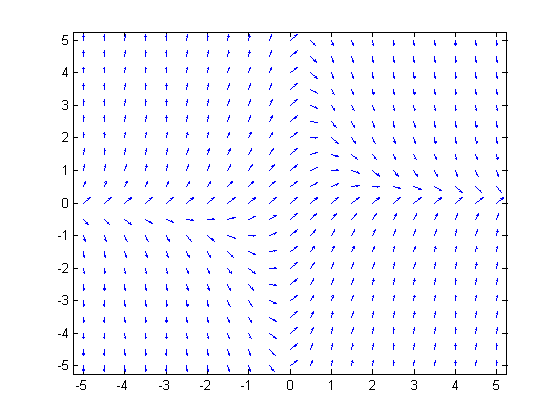
\includegraphics[width = 9cm]{WS_3}
\end{multicols}

\bigskip
\bigskip

\question
$\dfrac{dy}{dt} = \sin(t) \sin(y)$
\bigskip
\begin{multicols}{2}
\begin{parts}
\part
$y(0) = 1$
\part
$y(3) = 3$
\part
$y(1) = 0$
\part
$y(0) = -\dfrac{5}{2}$
\end{parts}
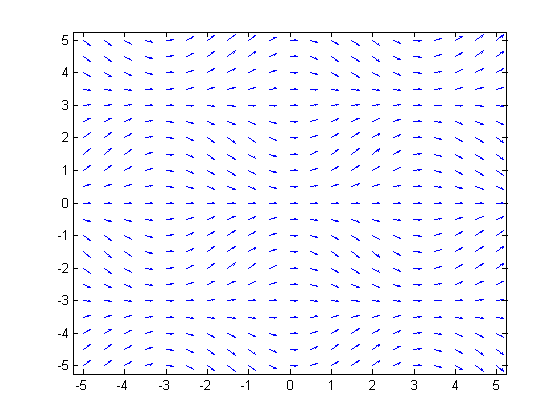
\includegraphics[width = 9cm]{WS_4}
\end{multicols}

\clearpage

\question
$\dfrac{dy}{dt} = 1 - \dfrac{y}{t}$
\bigskip
\begin{multicols}{2}
\begin{parts}
\part
$y(-\nicefrac{1}{2}) = 2$
\part
$y(\nicefrac{3}{2}) = 0$
\end{parts}
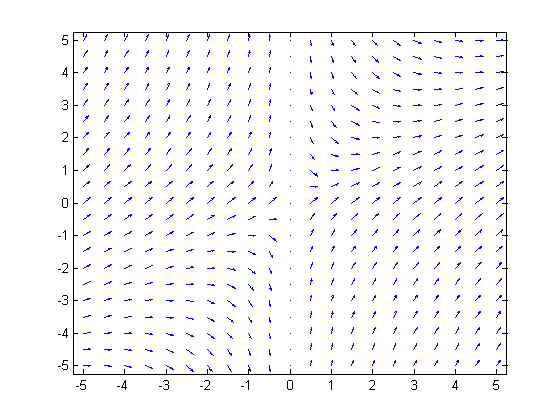
\includegraphics[width = 9cm]{WS_12}
\end{multicols}

\end{questions}

\end{document}
